\documentclass[11pt]{report}
\usepackage{amsmath, amssymb, amsthm}
\usepackage{geometry}
\usepackage{cite}
\geometry{margin=1in}

\usepackage{booktabs}
\usepackage{array}
\usepackage{enumitem}
\usepackage{lineno} 
\usepackage{xcolor} 
\newcommand{\gc}[1]{\textcolor{light-red}{#1}}
\newcommand{\blue}[1]{\textcolor[rgb]{0.00,0.00,1.00}{#1}}
\definecolor{light-gray}{gray}{0.96}
\definecolor{light-red}{rgb}{0.82, 0.1, 0.26}
\definecolor{light-smoke}{rgb}{0.96, 0.96, 0.93} 
\definecolor{light-olive}{rgb}{0.63, 0.57, 0.33}
\definecolor{light-azul}{rgb}{0.25, 0.41, 0.88}
\geometry{margin=1in}
\usepackage{hyperref}
 \usepackage{tikz,tabularx,booktabs,array}
 \usetikzlibrary{shapes,arrows,positioning,calc,shadows,backgrounds}
 
% \newcolumntype{Y}{>{\raggedright\arraybackslash}X}
 \usepackage{pgfplots}
\definecolor{rfcolor}{RGB}{51,122,183}
 \definecolor{processcolor}{RGB}{92,184,92}
 \definecolor{interfacecolor}{RGB}{217,83,25}
 \definecolor{datacolor}{RGB}{128,0,128}
 \usepackage[most]{tcolorbox}
 \newtcolorbox{verticalrulelist}[1][]{
 	enhanced,
 	skin=enhanced,
 	colback=white,
 	colframe=light-azul!90!black,
 	boxrule=0pt,
 	leftrule=2pt,
 	left=1em,
 	top=0.5em,
 	bottom=0.5em,
 	sharp corners,
 	#1
 }
\usepackage{pythonhighlight}
\lstdefinelanguage{turtle}
{
	columns=fullflexible,
	keywordstyle=\color{light-red},
	morekeywords={@prefix,@base,@forSome,@forAll,@keywords},
	morecomment=[l]{\#},
	tabsize=4, 
	alsoletter={-?}, % allowed in names
	morecomment=[s][light-azul]{<}{>},
	basicstyle=\ttfamily\color{black}, 
	%numberstyle=\color{black},
	morestring=[b][\color{black}]\", 
	background=\color{light-gray},
}

\begin{document}
	\section*{\begin{center}
		SDR-Based Spectrum Monitoring System for FM Broadcast Compliance Assessment
	\end{center}}
\paragraph*{Design Considerations for SDR-Based Monitoring Architectures}

\begin{itemize}
\item 
\textit{Reconfigurability and Flexibility:} The SDR platform must exhibit inherent reconfigurability to dynamically adjust signal processing parameters during monitoring operations. Since core functions---demodulation, detection thresholding, channel occupancy analysis, and compliance reporting---are virtualized in software rather than fixed in hardware, the system can adapt to evolving regulatory requirements, expand to adjacent frequency bands, or integrate advanced detection techniques (e.g., cyclostationary feature analysis, machine learning-based classification) via remote software updates without hardware modification.
	
\item 
\textit{Cost-Effectiveness:} By leveraging the HackRF One with embedded 	processors (DragonBoard~410c, Raspberry~Pi), the proposed architecture achieves persistent spectrum monitoring at substantially reduced cost versus traditional spectrum analyzers (\$10{,}000--\$50{,}000~USD per channel). With a target deployed cost of $\le$\$1000~USD per node---encompassing SDR, processor, RF 	front-end, enclosure, and deployment---the design enables order-of-magnitude scalability for distributed regulatory monitoring networks.
	
\item 
\textit{Remote Monitoring Capability:} The SDR-based system must transmit 
captured RF signal metadata, demodulated content, and compliance measurement 
results to a centralized server via IP-based networks, enabling regulatory 
personnel to monitor multiple FM broadcast stations from a central operations 
center. All data-in-transit must be protected using authenticated encryption 
(TLS~1.3 or higher, or IPsec-based VPN tunnels with AES-256-GCM). Access to 
the web-based monitoring interface shall be restricted to authenticated and 
authorized personnel via a role-based access control (RBAC) mechanism, with 
audit logging of all administrative actions.
	
	\item 
\textit{Multi-Station Monitoring:} The digital signal processing (DSP) 
pipeline shall support concurrent real-time demodulation and compliance 
analysis of a minimum of two FM broadcast channels on the target embedded 
platform. The system architecture shall be scalable to accommodate additional 
channels contingent upon available computational resources. Processing capacity 
shall be validated through empirical benchmarking on the target hardware prior 
to deployment, with the maximum sustainable concurrent channel count documented 
in the System Performance Specification.
	
\end{itemize}

\newpage
\paragraph*{Core Architectural Components}

\begin{figure}[!ht]
	\begin{center}
	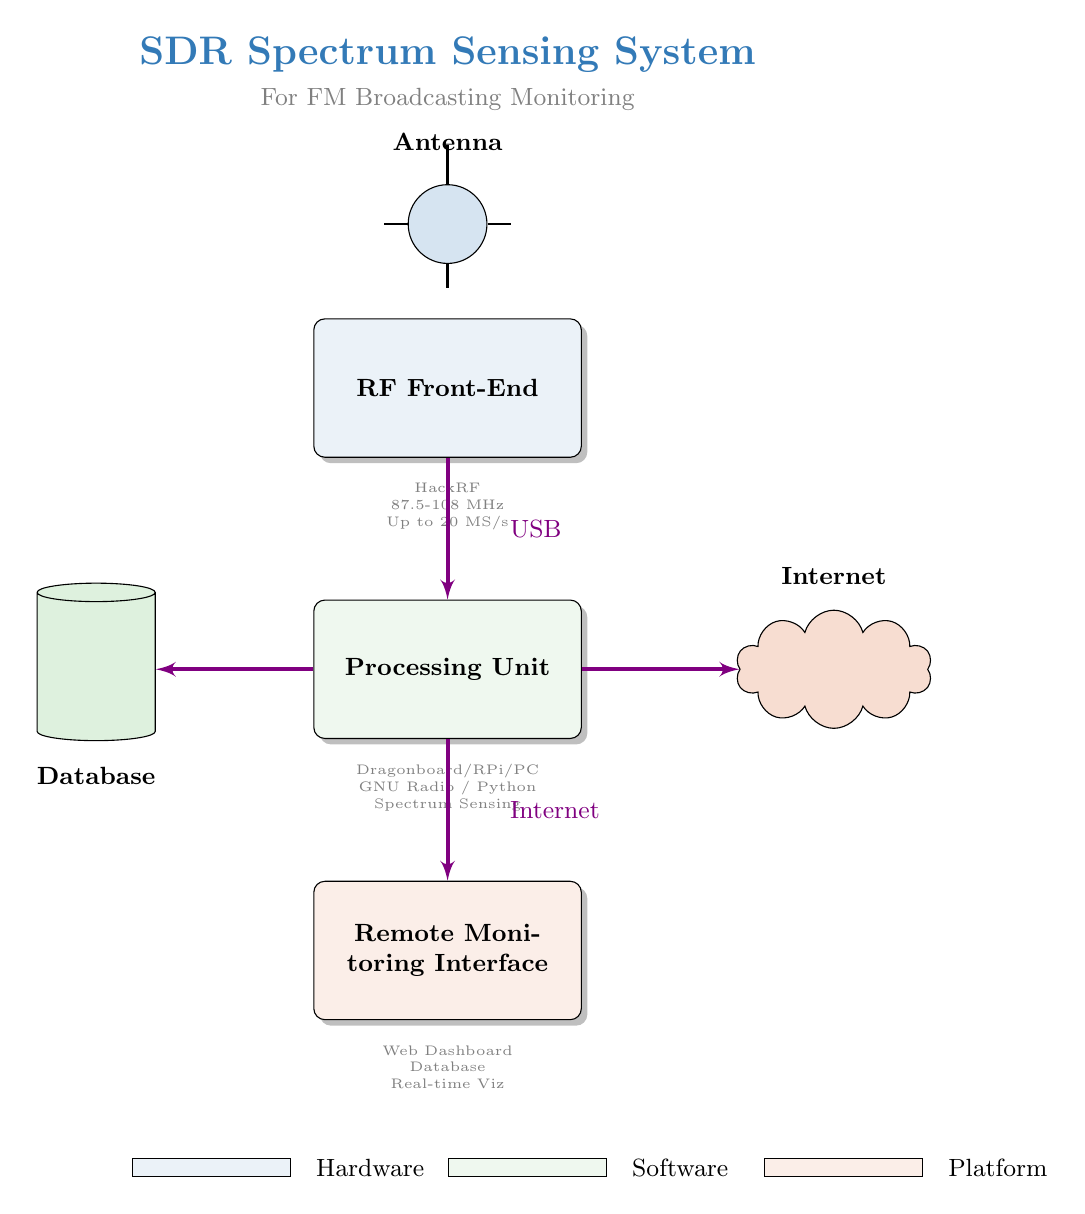
\begin{tikzpicture}[
	node distance=1.8cm,
	auto,
	>=latex',
	block/.style={
		rectangle,
		draw,
		fill=#1!10,
		text width=9em,
		text centered,
		rounded corners,
		minimum height=5em,
		drop shadow,
		font=\small\bfseries
	},
	block/.default=rfcolor,
	line/.style={
		draw,
		-latex',
		line width=1.5pt,
		color=datacolor
	},
	spec/.style={
		font=\tiny,
		text width=8em,
		text centered,
		color=gray
	}
	]
	
	% RF Front-End Block
	\node[block=rfcolor] (rf) {RF Front-End};
	\node[spec,below=0.2cm of rf] (rf-spec) {HackRF\\87.5-108 MHz\\Up to 20 MS/s};
	
	% Processing Unit Block
	\node[block=processcolor,below=of rf] (proc) {Processing Unit};
	\node[spec,below=0.2cm of proc] (proc-spec) {Dragonboard/RPi/PC\\GNU Radio / Python\\Spectrum Sensing};
	
	% Remote Monitoring Block
	\node[block=interfacecolor,below=of proc] (monitor) {Remote Monitoring Interface};
	\node[spec,below=0.2cm of monitor] (monitor-spec) {Web Dashboard\\Database\\Real-time Viz};
	
	% Connection Arrows
	\path[line] (rf) -- node[midway,right,font=\small] {\qquad USB} (proc);
	\path[line] (proc) -- node[midway,right,font=\small] {\qquad Internet} (monitor);
	
	% Antenna Icon
	\node[above=.69cm of rf, circle, draw, fill=rfcolor!20, minimum size=1cm] (antenna) {};
	\draw[thick] (antenna.north) -- ++(0,0.5);
	\draw[thick] (antenna.south) -- ++(0,-0.3);
	\draw[thick] (antenna.east) -- ++(0.3,0);
	\draw[thick] (antenna.west) -- ++(-0.3,0);
	\node[above=0.3cm of antenna, font=\small\bfseries] {Antenna};
	
	% Cloud/Internet Icon
	\node[right=2cm of proc, cloud, draw, fill=interfacecolor!20, 
	cloud puffs=10, minimum width=2.5cm, minimum height=1.5cm] (cloud) {};
	\node[above=0.2cm of cloud, font=\small\bfseries] {Internet};
	\path[line] (proc) -- (cloud);
	
	% Database Icon
	\node[left=2cm of proc, cylinder, draw, fill=processcolor!20, 
	shape border rotate=90, minimum height=2cm, minimum width=1.5cm] (db) {};
	\node[below=0.2cm of db, font=\small\bfseries] {Database};
	\path[line] (proc) -- (db);
	
	% Title
	\node[above=3.0cm of rf, font=\Large\bfseries, color=rfcolor] {SDR Spectrum Sensing System};
	\node[above=2.52cm of rf, font=\small, color=gray] {For FM Broadcasting Monitoring};
	
	% Legend
	\begin{scope}[shift={(-3,-9.9)}]
		\node[rectangle, draw, fill=rfcolor!10, minimum width=2cm, minimum height=0.15cm] (leg1) {};
		\node[right=0.2cm of leg1, font=\small] {Hardware};
		
		\node[rectangle, draw, fill=processcolor!10, minimum width=2cm, minimum height=0.15cm, right=2cm of leg1] (leg2) {};
		\node[right=0.2cm of leg2, font=\small] {Software};
		
		\node[rectangle, draw, fill=interfacecolor!10, minimum width=2cm, minimum height=0.15cm, right=2cm of leg2] (leg3) {};
		\node[right=0.2cm of leg3, font=\small] {Platform};
	\end{scope}
	
\end{tikzpicture}
\end{center}
	\caption{Core Architectural Design}
\end{figure}

\setlist[description]{font=\normalfont\itshape\textbullet\space}
\begin{description}
	\item[RF Front-End (Hardware Layer): ] 
 At the physical layer, a low-cost SDR receiver---the HackRF One---serves as the antenna-coupled RF front end. Its primary functions include: capturing incident RF energy in the VHF-II band (87.5--108~MHz), down-converting the signal to complex baseband via a heterodyne-conversion architecture, and digitizing it using a 8-bit ADC at up to 20~MS/s via USB 2.0. Instead of a direct-conversion architecture, the HackRF One uses a MAX2837 RF transceiver, which performs a two-stage heterodyne conversion — it is not a zero-IF direct-conversion device. This matters for the compliance monitoring application because direct-conversion receivers exhibit DC offset and IQ imbalance artifacts that degrade near-DC spectral measurements
However, sustained real-world throughput for the HackRF at the maximum rate is often lower than the theoretical limit due to USB 2.0 overhead and host buffering; practical deployments frequently cap at 10–15 MS/s without drops.
 
Critical performance parameters at this stage include instantaneous bandwidth, dynamic range, noise figure, and sampling rate, which collectively determine the signal integrity and measurement accuracy achievable for FM broadcast monitoring. A broadband antenna optimized for the VHF-II band couples to the SDR input, and a low-noise amplifier (LNA) may be integrated into the receive chain to improve system sensitivity and compensate for feedline attenuation in low-signal environments.

	\item[Signal Acquisition and Digitization: ] 
The SDR hardware streams raw complex baseband (I/Q) samples to the embedded host processor via a USB~2.0 high-speed interface. These quadrature samples represent the receiver's full instantaneous bandwidth---up to 20~MHz for the HackRF One---enabling capture of multiple FM broadcast channels (200~kHz spacing) within a single acquisition window. This wideband architecture provides a critical advantage over traditional narrowband receivers: rather than sequentially tuning to individual carriers, the system can simultaneously demodulate and analyze all FM stations falling within the instantaneous bandwidth, significantly reducing scan latency and enabling real-time correlation of spectral events across channels.

\item[Data Management and Reporting Layer: ]
Processed measurement results are persisted to a time-series database backend, structured around time-stamped records with metadata tags (frequency, location, station ID, compliance status). This schema enables efficient historical trending, statistical compliance analysis, and event-triggered alerting. A RESTful API and web-based dashboard provide remote access for regulatory personnel to query measurement data, visualize real-time spectrograms and spectral occupancy heatmaps, and generate audit-ready compliance reports aligned with regulatory templates (e.g., ITU-R SM.1880, FCC Part 73 technical rules). Automated alert mechanisms---configurable via threshold policies (absolute, statistical, or ML-based anomaly detection)---notify engineers via email, SMS, or webhook integrations when violations are detected, with escalation policies for critical events.

\item[Software Processing Engine:] 
The processing engine implements the end-to-end digital signal processing (DSP) pipeline for \emph{FM broadcast compliance monitoring}. Unlike communication-centric SDR applications, its primary output comprises \emph{auditable measurements, evidentiary records, 	and compliance reports}. 

The six-layer compliance monitoring pipeline is developed, embracing the following stages:
\begin{figure}[!ht]
	\centering
	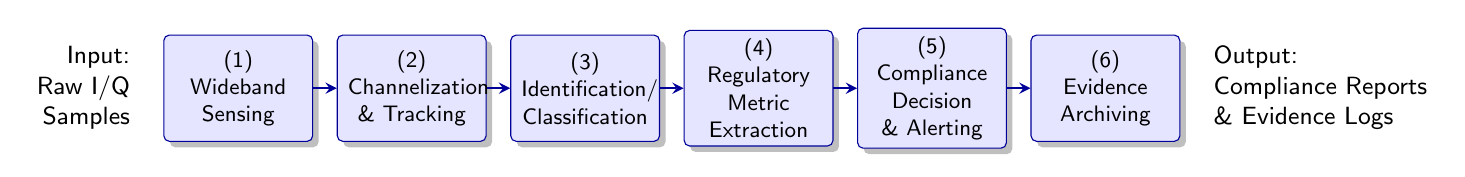
\begin{tikzpicture}[
		% Style definitions
		stage/.style={scale=0.9,
			rectangle,
			draw=blue!60!black,
			fill=blue!10,
			minimum width=2.1cm,
			minimum height=1.5cm,
			text width=1.8cm,
			align=center,
			font=\small\sffamily,
			rounded corners=2pt,
			drop shadow
		},
		arrow/.style={
			->,
			>=stealth,
			thick,
			blue!60!black
		},
		node distance=0.3cm
		]
		% Pipeline stages
		\node[stage] (S1) {(1)\\Wideband Sensing};
		\node[stage, right=of S1] (S2) {(2)\\Channelization \& Tracking};
		\node[stage, right=of S2] (S3) {(3)\\Identification/\\Classification};
		\node[stage, right=of S3] (S4) {(4)\\Regulatory Metric\\Extraction};
		\node[stage, right=of S4] (S5) {(5)\\Compliance Decision\\\& Alerting};
		\node[stage, right=of S5] (S6) {(6)\\Evidence Archiving};
		
		% Connection arrows
		\draw[arrow] (S1.east) -- (S2.west);
		\draw[arrow] (S2.east) -- (S3.west);
		\draw[arrow] (S3.east) -- (S4.west);
		\draw[arrow] (S4.east) -- (S5.west);
		\draw[arrow] (S5.east) -- (S6.west);
		
		% Optional: Input/Output labels
		\node[left=0.3cm of S1, font=\small\sffamily, align=right] {Input:\\Raw I/Q \\Samples};
		\node[right=0.3cm of S6, font=\small\sffamily, align=left] {Output:\\Compliance Reports\\\& Evidence Logs};
		
	\end{tikzpicture}
	\caption{SDR-based FM broadcast compliance monitoring processing pipeline. Raw I/Q samples flow through six sequential stages from wideband spectrum sensing to evidence archiving, enabling automated regulatory compliance assessment.}
	\label{fig:processing_pipeline}
\end{figure}

\end{description}
\paragraph*{Wideband Spectrum Sensing (Occupancy and Discovery).}
This stage estimates the Power Spectral Density (PSD) of received power across frequency to  (i)~discover active FM emissions, (ii)~maintain a time-stamped occupancy map  of the band, and (iii)~provide measurement features that feed station  tracking and compliance checks. Key outputs include detected station candidates (center frequency estimates), received signal strength indicators (RSSI), and activity timelines.

\begin{enumerate}
	\item \textit{Controlled Data Acquisition.}
	The SDR compliance monitoring architecture is characterized by 
	time-critical data ingress from the peripheral hardware to the host 
	processor via a USB interface. Discrepancies between the continuous 
	sampling rate and downstream processing or storage throughput can result 	in buffer overflows, excessive latency accumulation, or unbounded resource consumption. Consequently, the integration of a flow control mechanism---specifically backpressure propagation---is essential to regulate data flow, thereby ensuring system stability and deterministic operational behavior.
	
	\begin{verticalrulelist}
	\textbf{Experimental Set-up} \\
	The validated sensors are placed in close proximity to a common FM reference signal source, ensuring all HackRF One units are configured with identical settings and sample rates, to record data under identical environmental and operational conditions.
	\begin{itemize}[label=$\triangleright$, leftmargin=*, itemsep=0.3em]	
		\item All processing should be implemented in the software engine (GNU Radio/Python), ensuring compatibility with embedded targets (Dragonboard 410C, Raspberry Pi). 
		\item Benchmark the full pipeline on the target embedded hardware to verify that calibration overhead does not compromise the real-time monitoring requirement of ${\geq} 2$ simultaneous FM channels.
		
		\textit{Recommendation:} All hardware configuration parameters (gain, sample rate, antenna type) are documented to ensure reproducibility. The calibration procedure is executable as an automated script, triggered on-demand or on a scheduled basis, with results pushed to the central database.
		
	\end{itemize}
	
\end{verticalrulelist}
	\item \textit{Preprocessing.} The fidelity of the acquired measurement data is constrained by hardware impairments inherent to the HackRF One platform when used with the MAX2837 RF transceiver, which implements a two-stage heterodyne downconversion rather than a zero-IF direct-conversion path. Consequently, DC offsets, LO leakage, and I/Q imbalance manifest differently than in direct-conversion SDRs and must be addressed in the digital domain with awareness of the heterodyne architecture.
	
	\begin{verticalrulelist} \textbf{Experimental Set-up:} For real captures, the best hardware-aware workflow for HackRF One with MAX2837 is usually: tune slightly off-center, digitally shift if needed, and apply a time-domain DC blocker / mean removal on IQ, \begin{itemize}[label=$\triangleright$, leftmargin=*, itemsep=0.3em] \item \textbf{I/Q correction.} I/Q distortion in a heterodyne-based chain typically shows up as mirrored or ghost content around DC, and can also manifest as image lines near the downconverted IF. Implement per-channel I/Q imbalance calibration and compensation using reference signals, updating calibration as LO settings or center frequency change. \item \textbf{DC/LO leakage and center-spike correction.} In a two-stage downconversion path, DC-like spikes and LO leakage can appear at baseband (0 Hz) and at fixed offsets related to the IF downconversion stages. These artifacts are not guaranteed to be fixed at 0 Hz across all tunings; their amplitude and location can vary with tuning. Apply a time-domain DC blocker and a dynamic, channel-specific DC notch near 0 Hz, complemented by LO-leakage calibration to suppress persistent spurs. \item \textbf{Comb-like spikes.} Comb-like, evenly spaced spikes can arise from sampling clock/quantization artifacts or external intermodulation, and may be exacerbated by I/Q imbalance or LO spurs. Use clock-aware filtering with notches at known clock-harmonic offsets and robust spectral preprocessing to distinguish genuine emissions from artifacts. Maintain a log of identified spurs for traceability. \end{itemize} \end{verticalrulelist}
\item \textit{Spectral Parameter Estimation.}
Given a Power Spectral Density (PSD) estimate $\widehat{S}_{x}(f)$ over 
a band of interest, derive the following band-level features:
	
	\begin{figure}[!ht]
		\centering
		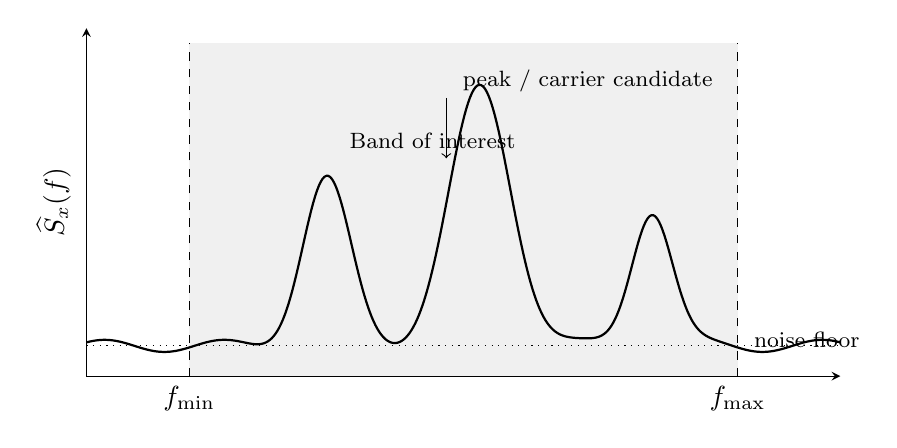
\begin{tikzpicture}
			\begin{axis}[
				width=0.92\linewidth,
				height=6.0cm,
			%	xlabel={$f$},
				ylabel={$\widehat{S}_{x}(f)$},
				xmin=-110, xmax=110,
				ymin=0, ymax=1.15,
				axis lines=left,
				xtick=\empty, ytick=\empty,
				clip=false,
				domain=-110:110,
				samples=400,
				enlargelimits=false
				]
				
				% --- Band of interest markers ---
				\draw[dashed] (axis cs:-80,0) -- (axis cs:-80,1.10);
				\draw[dashed] (axis cs: 80,0) -- (axis cs: 80,1.10);
				
				\node[anchor=north] at (axis cs:-80,0) {$f_{\min}$};
				\node[anchor=north] at (axis cs: 80,0) {$f_{\max}$};
				
				% --- Shaded band of interest ---
				\path[fill=black, fill opacity=0.06, draw=none]
				(axis cs:-80,0) rectangle (axis cs:80,1.10);
				
				\node[anchor=south] at (axis cs:-9,0.72) {\footnotesize Band of interest};
				
				% --- PSD curve (stylized: noise floor + three emissions) ---
				\addplot[thick]
				{0.10
					+ 0.55*exp(-((x+40)^2)/(2*7^2))
					+ 0.85*exp(-((x-5 )^2)/(2*9^2))
					+ 0.45*exp(-((x-55)^2)/(2*6^2))
					+ 0.02*cos(deg(0.18*x))};
				
				% --- Optional: label one peak ---
				\draw[->] (axis cs:-5,0.92) -- (axis cs:-5,0.72);
				\node[anchor=west] at (axis cs:-3,0.975) {\footnotesize peak / carrier candidate};
				
				% --- Noise floor cue ---
				\draw[dotted] (axis cs:-110,0.10) -- (axis cs:110,0.10);
				\node[anchor=west] at (axis cs:82,0.12) {\footnotesize noise floor};
				
			\end{axis}
		\end{tikzpicture}
		\caption{Illustration of a PSD estimate $\widehat{S}_{x}(f)$ of the received wideband complex I/Q over a frequency band of interest $[f_{\min},f_{\max}]$, showing a noise floor and multiple detected emissions.}
	\end{figure}
	
	\begin{verticalrulelist}
		\textbf{Experimental Set-up} \\
		\begin{itemize}[label=$\triangleright$, leftmargin=*, itemsep=0.3em]
			\item \textit{Noise Floor Estimation} 
			
			\item \textsl{Power at specific frequencies:} $\widehat{S}_{x}(f_k)$ 
			for selected $f_k$ (e.g., nominal channel centers).
			\item \textit{Peak frequency:} $f_{\text{pk}} \triangleq 
			\arg\max_{f}\,\widehat{S}_{x}(f)$ (candidate carrier location).
			\item \textsl{Occupied bandwidth:} $B_{\text{occ}}$ defined as the 
			smallest bandwidth around a center $f_c$ that contains a prescribed 
			fraction of in-band power (e.g., $99\%$), or equivalently via a 
			thresholded support set.
			\item \textsl{Center frequency (spectral centroid):} $f_{\text{cent}}$ 
			interpreted as a power-weighted mean frequency over the analyzed band.
			\item \textsl{SNR proxy:} Robust estimate of in-band signal power 
			relative to a noise-floor estimate, producing $\widehat{\mathrm{SNR}}$ 
			for detection confidence and alert thresholds.
		\end{itemize}
	\end{verticalrulelist}
	\item \textit{Occupancy Detection and Band Discovery.}
	Convert $\widehat{S}_{x}(f)$ into a binary (or probabilistic) occupancy 
	map by comparing against a noise-floor estimate $\widehat{N}(f)$:
	\[
	\mathcal{O}(f)=\mathbf{1}\{\widehat{S}_{x}(f) > \widehat{N}(f)+\gamma\},
	\]
	where $\gamma$ is a configurable margin (in dB). Connected occupied 
	regions define candidate emissions; their centers, peak locations, and 
	widths provide initial station candidates for downstream channelization 
	and tracking.
	
	\begin{verticalrulelist}
		\textbf{Experimental Set-up:}    compliance-oriented and signal-quality features are extracted from each sensor's normalized data:
	
	\begin{itemize}[label=$\triangleright$, leftmargin=*, itemsep=0.3em]
		\item \textit{Standard spectral features:} Spectral flatness, SNR proxy, occupied bandwidth ($B_{\text{occ}}$), carrier frequency error/drift, spectral centroid ($f_{\text{cent}}$)\[
		f_{\text{cent}} \triangleq {\int f\,\widehat{S}_{x}(f)\,df}\big{/}{\int \widehat{S}_{x}(f)\,df},
		\] \textit{Power at specific frequencies} \textit{Peak frequency} \textit{Occupied bandwidth} \textit{Center frequency (spectral centroid)}
		\item \textit{FM-specific features:} 19~kHz pilot tone SNR, MPX spectral structure integrity (presence of 38~kHz stereo subcarrier, 57~kHz RDS), deviation profile consistency. \textit{SNR proxy:} estimate in-band signal power relative to a noise-floor estimate (median/robust fit outside detected carriers), producing $\widehat{\mathrm{SNR}}$ for detection confidence and alert thresholds.
	\end{itemize}
	\textit{Recommendation:} Prioritize features ``Compliance Feature Extraction'' module to ensure regulatory relevance. Standardize all features (zero-mean, unit-variance) before downstream similarity computations.
	\end{verticalrulelist}
	\item \textit{Quantitative Reconstruction of PSD.}
	When the PSD is degraded by noise, short observation windows, or coarse 
	resolution, apply reconstruction techniques to improve the stability of 
	the occupancy map and derived features. Examples include: (i)~smoothing 
	or averaging across time, (ii)~interpolation across frequency bins, and 
	(iii)~model-based fitting for the noise floor and/or emission shapes. 
	This stage must preserve auditability by logging parameters and 
	reconstruction settings used for each reported estimate.

	\item \textit{Demodulation-Assisted Verification \& Station Identification.}
	After candidate emissions are discovered from $\widehat{S}_{x}(f)$, each 
	candidate channel is \emph{isolated and decimated} (channelization 
	$\rightarrow$ narrowband I/Q) and a lightweight FM demodulation stage is 
	applied to:
	
 	\begin{figure}[!ht]
		\centering
		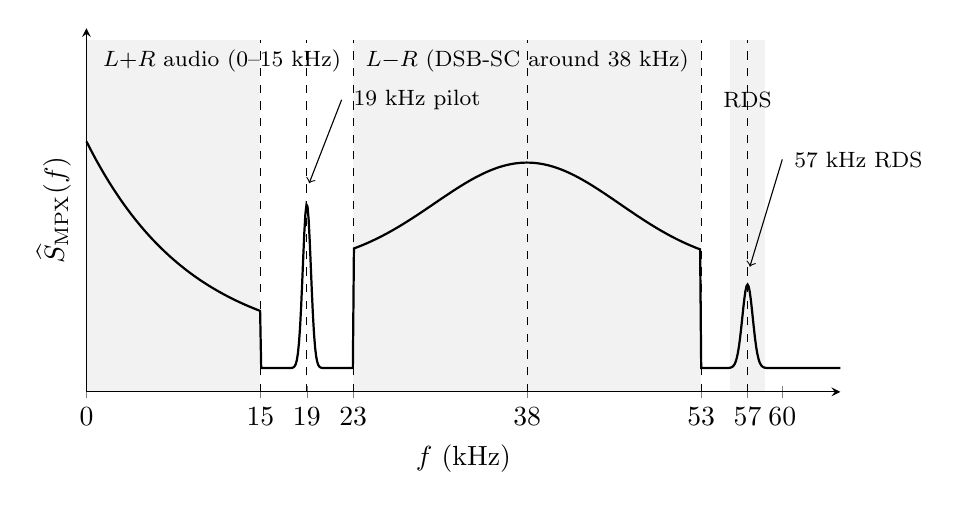
\begin{tikzpicture}
			\begin{axis}[
				width=0.92\linewidth,
				height=6.2cm,
				xlabel={$f$ (kHz)},
				ylabel={$\widehat{S}_{\mathrm{MPX}}(f)$},
				xmin=0, xmax=65,
				ymin=0, ymax=1.22,
				axis lines=left,
				xtick={0,15,19,23,38,53,57,60},
				ytick=\empty,
				clip=false,
				samples=700,
				domain=0:65,
				enlargelimits=false
				]
				
				% Shaded regions for main MPX components
				\path[fill=black, fill opacity=0.05, draw=none]
				(axis cs:0,0) rectangle (axis cs:15,1.18);
				\node[anchor=south west] at (axis cs:0.6,1.04) {\footnotesize $L{+}R$ audio (0--15 kHz)};
				
				\path[fill=black, fill opacity=0.05, draw=none]
				(axis cs:23,0) rectangle (axis cs:53,1.18);
				\node[anchor=south] at (axis cs:38,1.04) {\footnotesize $L{-}R$ (DSB-SC around 38 kHz)};
				
				\path[fill=black, fill opacity=0.05, draw=none]
				(axis cs:55.5,0) rectangle (axis cs:58.5,1.18);
				\node[anchor=south] at (axis cs:57,0.92) {\footnotesize RDS};
				
				% MPX PSD curve (stylized). Exponent clipping avoids "Dimension too large".
				\addplot[thick]
				{
					0.08
					+ (x<=15)*(0.70*exp(-x/9.0) + 0.06*cos(0.65*x))
					+ 0.55*exp(max(-50, -((x-19)^2)/(2*(0.35^2)))) % 19 kHz pilot (narrow)
					+ (x>=23)*(x<=53)*(0.30 + 0.35*exp(-((x-38)^2)/(2*(8.0^2))) + 0.04*cos(0.80*(x-23)))
					+ 0.28*exp(max(-50, -((x-57)^2)/(2*(0.45^2)))) % 57 kHz RDS (narrow)
				};
				
				% Guide lines
				\draw[dashed] (axis cs:15,0) -- (axis cs:15,1.18);
				\draw[dashed] (axis cs:19,0) -- (axis cs:19,1.18);
				\draw[dashed] (axis cs:23,0) -- (axis cs:23,1.18);
				\draw[dashed] (axis cs:38,0) -- (axis cs:38,1.18);
				\draw[dashed] (axis cs:53,0) -- (axis cs:53,1.18);
				\draw[dashed] (axis cs:57,0) -- (axis cs:57,1.18);
				
				% Labels
				\draw[->] (axis cs:22.0,0.98) -- (axis cs:19.2,0.70);
				\node[anchor=west] at (axis cs:22.2,0.98) {\footnotesize 19 kHz pilot};
				
				\draw[->] (axis cs:60.0,0.78) -- (axis cs:57.2,0.42);
				\node[anchor=west] at (axis cs:60.2,0.78) {\footnotesize 57 kHz RDS};
				
			\end{axis}
		\end{tikzpicture}
		\caption{Demodulated baseband spectrum (post-demod) of the audio/composite (MPX) after FM discriminator, centered at 0 Hz audio, with features like 19 kHz pilot, 38 kHz stereo subcarrier, and possibly 57 kHz RDS.		
		}
	\end{figure}
\begin{itemize}
	\item \textsl{Confirm emission type:} Verify that the detected 
	occupancy corresponds to an FM broadcast-like signal (reject 
	interferers and non-broadcast emissions).
	\item \textsl{Extract identification cues:} Detect the 19~kHz stereo 
	pilot and optionally decode Radio Data System (RDS) to obtain station 
	metadata (e.g., PI, PS, PTY when available).
	\item \textsl{Support evidence generation:} Produce short, 
	time-stamped \emph{audio snippets} and/or \emph{RDS logs} linked to 
	occupancy events for audits and investigations.
	\item \textsl{Enable demodulation-derived metrics (optional):} 
	Compute modulation or deviation-related indicators when required by 
	the compliance rule set.
\end{itemize}

% 	 \item \textit{Pairwise Similarity Metrics} \\
% Compute inter-sensor similarity features to quantify agreement:
% 	\begin{itemize}[label=$\circ$, leftmargin=*, itemsep=0.2em]
% 	 \item Cross-correlation of PSD estimates over the FM band.
% 	 \item Euclidean or Mahalanobis distance in the standardized feature space.
% 	\item Coherence metrics or dynamic time warping (DTW) for temporal alignment of signal-level trends.
% 	 \end{itemize}
% 	 \textit{Recommendation:} Document the similarity metric choice and its parameters in the system specification for reproducibility.
%
% \item \textit{Dimensionality Reduction \& Clustering} \\
% Perform Principal Component Analysis (PCA) on the concatenated feature set (per-sensor features + pairwise similarities) to identify dominant modes of variation. Assess cluster centroids in the reduced feature space to identify groups of consistent sensors.
% 
% \textit{Recommendation:} Report the cumulative variance explained by the first $k$ principal components. If PC1 explains $>90\%$ of variance, it likely represents the ``true signal''; subsequent components may capture sensor-specific artifacts. Retain reconstruction parameters for auditability 
% \item \textit{Consensus Assessment \& Tagging} \\
%Evaluate the proximity of each sensor's feature vector to the principal centroid(s) in the PCA space. Sensors within a defined confidence region (e.g., $2\sigma$ Mahalanobis distance) are flagged as \textit{Verified}; those exceeding the threshold are tagged \textit{Unverified} and excluded from compliance reporting until recalibrated.
% 
%\textit{Recommendation:} Integrate this tagging logic into the Data Management Layer (PDF Section~2) so that only \textit{Verified} sensors contribute to automated compliance alerts and regulatory reports.

\end{enumerate}
%\newpage
%\begin{center}
%	\textbf{\Large RF/FM Data Loading \& Diagnostics}
%\end{center}
%\vspace{0.5cm}
%
%\blue{DatasetFM-v0}
%
%\vspace{0.5cm}
%
%\textbf{1. Load Integrity Checking of CSV data}
%\begin{itemize}
%	\item File-Level Integrity
%	\begin{itemize}
%		\item Encoding, delimiter, header validation
%		\item Empty / unreadable file detection
%	\end{itemize}
%	\item Row-Level Integrity
%	\begin{itemize}
%		\item NaN handling
%		\item Duplicate row detection
%		\item Type coercion validation
%		\item Cross-file schema consistency
%	\end{itemize}
%	\item Validate value consistency 
%	\begin{itemize}
%		\item Pxx: range, length. Alignment check between \texttt{Pxx} and \texttt{Loc}
%		\item Loc collection: range, length (add missing)
%	\end{itemize}
%	
%\end{itemize}
%\vspace{0.3cm}
%\textbf{2. Load Dataset Report}
%\begin{itemize}
%	\item Global Aggregate Statistics
%	\begin{itemize}
%		\item Column Consistency Check
%		\item Data Type \& Sample Preview
%		\item Row Index Range Validation
%		\item Per-Node Shape Information
%	\end{itemize}
%	\item Visual and Export Summary
%	\begin{itemize}
%		\item Record Integrity Visualization
%		\item Memory Usage Visualization
%		\item Exportable summary dictionary (define keys)
%		\item Audit log of all checks with pass/fail status
%	\end{itemize}
%\end{itemize}
%\vspace{0.3cm}
%\textbf{3. RF/FM Node Diagnostics}
%\begin{itemize}
%	\item PSD diagnostics for anomaly detection in nodes \blue{DatasetFM-v1}
%	
%	Pxx Histogram shape Analysis, including 
%	Correlation Matrix of PSD Histogram Shapes for quantifying how similar the distribution patterns of Power Spectral Density (PSD) values are across different nodes, and estimation of Cumulative Score ranking is finally computed.
%	\begin{itemize}
%		\item Recorded data
% \item Preprocessing: 
% 
% For real captures, the best hardware-aware workflow for HackRF One is usually:
% 
% tune slightly off-center,
% 
% digitally shift if needed,
% 
% apply a time-domain DC blocker / mean removal on IQ,
% 
% then compute the PSD.
% 
% %If you want, I can also give you the matching IQ-domain DC blocker for HackRF captures so the center spike is reduced before PSD estimation.
%	\end{itemize}
%\end{itemize}
%
%\begin{enumerate}	
%	\item \textsl{Channelization and Station Tracking.} 
%	Isolate each detected station using digital channelization 
%	(e.g., FFT-based or Polyphase Filter Bank~(PFB) channelizer) and track 
%	(i)~center frequency drift, (ii)~signal level trends, and 
%	(iii)~continuity or outage events over time.
%	
%	\item \textsl{Signal Identification and Classification.} 
%	Classify emissions to verify broadcast service status: confirm FM broadcast 
%	characteristics (e.g., deviation profile), detect the stereo pilot tone 
%	(19~kHz), and optionally decode the Radio Data System (RDS) for station 
%	identification metadata. This step supports \emph{station attribution} and 
%	reduces false alarms from non-broadcast interferers.
%	
%	\item \textsl{Regulatory Metric Extraction.} 
%	Compute regulatory-relevant metrics per station, such as occupied bandwidth 
%	(OBW), Adjacent Channel Power Ratio (ACPR), spurious emissions, and carrier 
%	frequency error. These features feed rule-checking algorithms and reporting 
%	modules.
%	
%	\item \textsl{Compliance Decision Logic and Alerting.} 
%	Apply configurable decision rules (thresholds, spectral masks, persistence 
%	criteria) to flag potential non-compliance events, generate alerts, and 
%	annotate events with confidence scores.
%	
%	\item \textsl{Evidence Archiving and Reporting.} 
%	Store time-stamped measurement summaries and optional recorded evidence 
%	segments (I/Q samples or demodulated audio) with cryptographic integrity 
%	controls (e.g., hashing or digital signatures). Generate periodic compliance 	reports (daily/weekly) plus event-driven incident logs.
%\end{enumerate}


\end{document}


NB
I am developing an spectrum sensing system, based on SDR.
The attached notebook assesses the measured data quality of the nodes.
Due to the restrictions of the selected HackRF one board, in terms of center spike and I/Q distortion,  the quality of measure PSD is as follows:

Provide an algorithm for estimating the center frequency to add to the working notebook to evualuate the quality of each sensor.

\item \gc{Data curation.} \\ 
It provides ongoing management of data throughout its lifecycle—from creation to preservation—to ensure it remains findable, accessible, interoperable, and reusable (FAIR). It involves cleaning, structuring, annotating with metadata, and validating data to improve quality, prevent bias, and maximize its long-term value.

"Assume the role of an expert RF and Systems Engineer. I am developing a Software-Defined Radio (SDR) system for RF spectrum monitoring and FM broadcast regulatory compliance. Below is a reference guide we authored to assess the measurement fidelity and calibration quality of our sensor array. Please review the following text for structural consistency, logical coherence, and technical rigor"